
%%%%%%%%%%%%%%%%%%%%%%%%%%%%%%%%%%%%%%%%%%%%%%%%%%%%%%%%%%%%%%%%%%%%%%%%%%%%%%%%%%%%%%%
%%%%%%%%%%%%%%%%%%%%%%%%%%%%%%%%%%%%%%%%%%%%%%%%%%%%%%%%%%%%%%%%%%%%%%%%%%%%%%%%%%%%%%%
% 
% This top part of the document is called the 'preamble'.  Modify it with caution!
%
% The real document starts below where it says 'The main document starts here'.

\documentclass[12pt]{article}

\usepackage{amssymb,amsmath,amsthm}
\usepackage[top=1in, bottom=1in, left=1.25in, right=1.25in]{geometry}
\usepackage{fancyhdr}
\usepackage{enumerate}
\usepackage{listings}
\usepackage{graphicx}
\usepackage{float}

% Comment the following line to use TeX's default font of Computer Modern.
\usepackage{times,txfonts}



\makeatletter
\renewcommand*\env@matrix[1][*\c@MaxMatrixCols c]{%
  \hskip -\arraycolsep
  \let\@ifnextchar\new@ifnextchar
  \array{#1}}
\makeatother

\newtheoremstyle{homework}% name of the style to be used
  {18pt}% measure of space to leave above the theorem. E.g.: 3pt
  {12pt}% measure of space to leave below the theorem. E.g.: 3pt
  {}% name of font to use in the body of the theorem
  {}% measure of space to indent
  {\bfseries}% name of head font
  {:}% punctuation between head and body
  {2ex}% space after theorem head; " " = normal interword space
  {}% Manually specify head
\theoremstyle{homework} 

% Set up an Exercise environment and a Solution label.
\newtheorem*{exercisecore}{Exercise \@currentlabel}
\newenvironment{exercise}[1]
{\def\@currentlabel{#1}\exercisecore}
{\endexercisecore}

\newcommand{\localhead}[1]{\par\smallskip\noindent\textbf{#1}\nobreak\\}%
\newcommand\solution{\localhead{Solution:}}

%%%%%%%%%%%%%%%%%%%%%%%%%%%%%%%%%%%%%%%%%%%%%%%%%%%%%%%%%%%%%%%%%%%%%%%%
%
% Stuff for getting the name/document date/title across the header
\makeatletter
\RequirePackage{fancyhdr}
\pagestyle{fancy}
\fancyfoot[C]{\ifnum \value{page} > 1\relax\thepage\fi}
\fancyhead[L]{\ifx\@doclabel\@empty\else\@doclabel\fi}
\fancyhead[C]{\ifx\@docdate\@empty\else\@docdate\fi}
\fancyhead[R]{\ifx\@docauthor\@empty\else\@docauthor\fi}
\headheight 15pt

\def\doclabel#1{\gdef\@doclabel{#1}}
\doclabel{Use {\tt\textbackslash doclabel\{MY LABEL\}}.}
\def\docdate#1{\gdef\@docdate{#1}}
\docdate{Use {\tt\textbackslash docdate\{MY DATE\}}.}
\def\docauthor#1{\gdef\@docauthor{#1}}
\docauthor{Use {\tt\textbackslash docauthor\{MY NAME\}}.}
\makeatother

% Shortcuts for blackboard bold number sets (reals, integers, etc.)
\newcommand{\Reals}{\ensuremath{\mathbb R}}
\newcommand{\Nats}{\ensuremath{\mathbb N}}
\newcommand{\Ints}{\ensuremath{\mathbb Z}}
\newcommand{\Rats}{\ensuremath{\mathbb Q}}
\newcommand{\Cplx}{\ensuremath{\mathbb C}}
%% Some equivalents that some people may prefer.
\let\RR\Reals
\let\NN\Nats
\let\II\Ints
\let\CC\Cplx

%%%%%%%%%%%%%%%%%%%%%%%%%%%%%%%%%%%%%%%%%%%%%%%%%%%%%%%%%%%%%%%%%%%%%%%%%%%%%%%%%%%%%%%
%%%%%%%%%%%%%%%%%%%%%%%%%%%%%%%%%%%%%%%%%%%%%%%%%%%%%%%%%%%%%%%%%%%%%%%%%%%%%%%%%%%%%%%
% 
% The main document start here.

% The following commands set up the material that appears in the header.
\doclabel{STAT 401: Homework 3}
\docauthor{Stefano Fochesatto}
\docdate{\today}

\begin{document}

\begin{exercise}{1} Do problem 2.1. Complete 2.1.1, 2.1.2, and only do the first two sentences of 2.1.3.\\
   \begin{enumerate}
     \item[2.1.1] Draw a scatterplot of $wt$ on the vertical axis versus $ht$ on the horizontal axis. On the basis of this plot, 
     does a simple linear regression model make sense for these data? Why or why not?\\
     \begin{figure}[H]
      \begin{center}
      \caption{Height vs Weight Scatter Plot}
      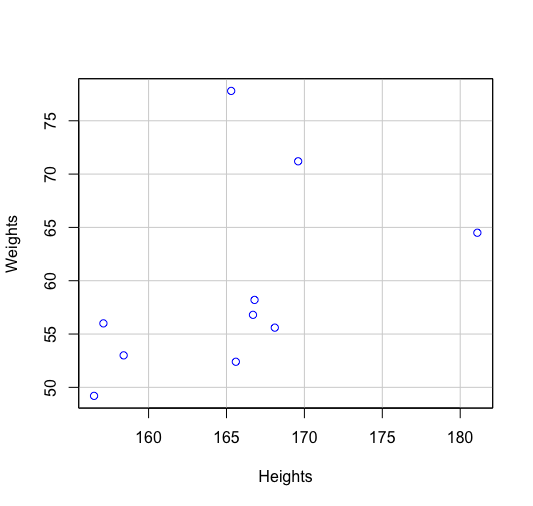
\includegraphics[width=.66\textwidth]{Rplot.png}
      \end{center}
  \end{figure}
  \textbf{Code:}
        \begin{center}
        \lstinputlisting{r1.txt}
        \end{center} 
  The data does not look ideal for a linear regression model. You can see that as the 
  height increase we experience more variance in the weight values. A linear regression model 
  assumes constant variance.
  \newpage

  \item[2.1.2] Show that $\bar{x} = 165.52$, and $\bar{y} = 59.37$, $SXX = 472.08$, $SYY = 731.96$, and 
  $SXY = 274.79$. Compute the estimates of the slope and intercept for the regression of $Y$ on $X$. 
  Draw the fitted line on you scatterplot.  \\
  \solution Calculating $\bar{x}$ and $\bar{y}$ just applying the mean formula on the data. 
  Computing $SXX$, $SYY$, and $SXY$ involves using the following formula, 
  \begin{equation*}
    SXX = \sum(x_i - \bar{x})^2,
  \end{equation*}
  \begin{equation*}
    SYY = \sum(y_i - \bar{y})^2,
  \end{equation*}
  \begin{equation*}
    SXY = \sum(x_i - \bar{x})(y_i - \bar{y})^2.
  \end{equation*}
  Given our values we can finally solve for $\hat{\beta}_0$ and $\hat{\beta}_1$
  \begin{equation*}
    \hat{\beta}_1 = \dfrac{SXY}{SXX} = \dfrac{274.786}{472.076} = 0.58208
  \end{equation*}
  \begin{equation*}
    \hat{\beta}_2 =  \bar{y} -  \bar{x}\hat{\beta}_1 = 59.37 - 165.52(0.58208) = -36.97588
  \end{equation*}

  \begin{figure}[h]
    \begin{center}
    \caption{Height vs Weight Scatter Plot with Regression}
    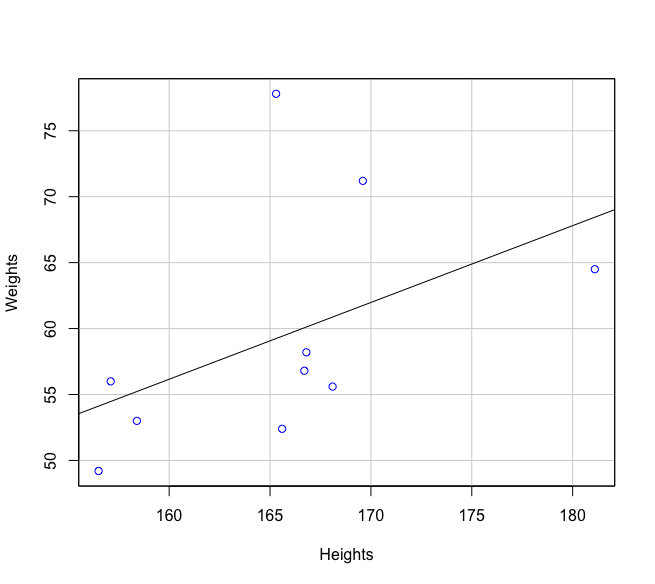
\includegraphics[width=.66\textwidth]{Rplot2.png}
    \end{center}
\end{figure}

  \textbf{Code:}
  \begin{center}
  \lstinputlisting{r2.txt}
  \end{center} 
  \newpage

  \item[2.1.3] Obtain the estimate of $\sigma^2$ and find the estimated standard errors of 
  $\hat{\beta}_0$ and $\hat{\beta}_1$. Also find the estimated covariance between  $\hat{\beta}_0$ and $\hat{\beta}_1$.\\ 
  \solution Recall that our estimator for $\sigma^2$ is computed by, 
  \begin{equation*}
    \hat{\sigma}^2 = \dfrac{RSS}{n - 2} = \dfrac{\sum(y_i - \hat{y}_i)^2}{n-2} = 71.5142
  \end{equation*}
  Now recall the formulas for computing the standard errors of $\hat{\beta}_0$ and $\hat{\beta}_1$, 
  \begin{equation*}
    SE(\hat{\beta_0}) = \sqrt{\hat{\sigma}^2\left(\frac{1}{n} + \frac{\bar{x}^2}{SXX}\right)} =  \sqrt{71.5142\left(\frac{1}{10} + \frac{165.52^2}{472.076}\right)} \approx 64.478
  \end{equation*}
  \begin{equation*}
    SE(\hat{\beta_1}) = \sqrt{\hat{\sigma}^2 \frac{1}{SXX}} =  \sqrt{71.5142 \frac{1}{472.076}} \approx 0.389
  \end{equation*}
  Solving for the estimated covariance, 
  \begin{equation*}
    Cov(\hat{\beta_0}, \hat{\beta_1}) = -\hat{\sigma}^2 \frac{\bar{x}}{SXX} = -71.5142 \frac{165.52}{472.076} \approx 25.0744
  \end{equation*}
   \end{enumerate}
\end{exercise}
\newpage

\begin{exercise}{2} For the data set in problem 2.1, do the following, 
  \begin{enumerate}[a.]
    \item Write out the simple linear regression model, including the mean and the variance function.\\
    \solution From the previous problem we have already computed the simple linear regression model, 
    \begin{equation*}
      y = \hat{\beta_0} + \hat{\beta_1}x = -36.976 +  0.582x
    \end{equation*}
    We also know that the expected value and mean functions, 
    \begin{equation*}
      E(Y) = -36.976 +  0.582x,
    \end{equation*}
    \begin{equation*}
      V(E(Y)) =  \hat{\sigma}^2 \left(\frac{1}{n} + \frac{(x - \bar{x})^2}{SXX}\right) = 71.5142 \left(\frac{1}{10} \frac{(x - 165.52)^2}{472.08}\right).
    \end{equation*}
    \vspace{.15in}

    \item Interpret the intercept and slope estimates you obtained above.\\
    \solution The intercept of our linear regression model suggests that on average when someone is 
    0 centimeters then they weigh approximately negative 36 kilos. The slope of our linear regression model
    suggests that for every 1 centimeter of height we can expect the weight to increase by approximately 0.6 kilos. 
    \vspace{.15in}

    \item What does it mean when we call the fitted model the "best" in other words what is the idea behind OLS?\\
    \solution The fitted (OLS)model is created by minimizing the residual sum of squares(RSS) function. 
    \begin{equation*}
      RSS(\hat{\beta_0}, \hat{\beta_1}) = \sum_{i = 1}^n (y_i - \hat{\beta_0} + \hat{\beta_1}x_i)^2
    \end{equation*}
    The idea behind this is, if the residual is a good estimate for the error or inaccuracy in the model, it makes sense to 
    create a model by minimizing the residual. Our (OLS) model give the smallest residual or highest accuracy, so it is the 'best' fit for the 
    data. 
    \vspace{.15in}

    \item What does it mean to say that the OLS estimators are linear?\\
    \solution We say that the OLS estimators are linear because they are produced via a linear combination of 
    $y_i$. More accurately we would say that the OLS estimators are linear with respect to the response variable.
    \vspace{.15in}

    \item Using the fitted model, predict the weight of a person from this population who is 171.0 cm tall. 
    \solution
    \begin{equation*}
      -36.976 +  0.582(171.0cm) = 62.546kg
    \end{equation*}
  \end{enumerate}
\end{exercise}
\newpage

\begin{exercise}{3} For the data set brains in the alr4 library, do the following,\\
  \begin{enumerate}[a.]
    \item Fit the simple linear regression model using log(BrainWT) as the response and log(BodyWT)
    as the predictor. Report the estimated slope and residual standard error of the fitted model.\\
    \solution Fitting the simple linear regression using r we get the following,
    \begin{equation*}
      \hat{\beta_1} = 0.75169
    \end{equation*}
    \begin{equation*}
      \hat{\beta_0} = 2.13479 
    \end{equation*}
    \begin{equation*}
     RSE = 0.6943
    \end{equation*}

  \begin{figure}[h]
    \begin{center}
    \caption{Log Body-Weight vs Log Brain-Weight Scatter Plot with Regression}
    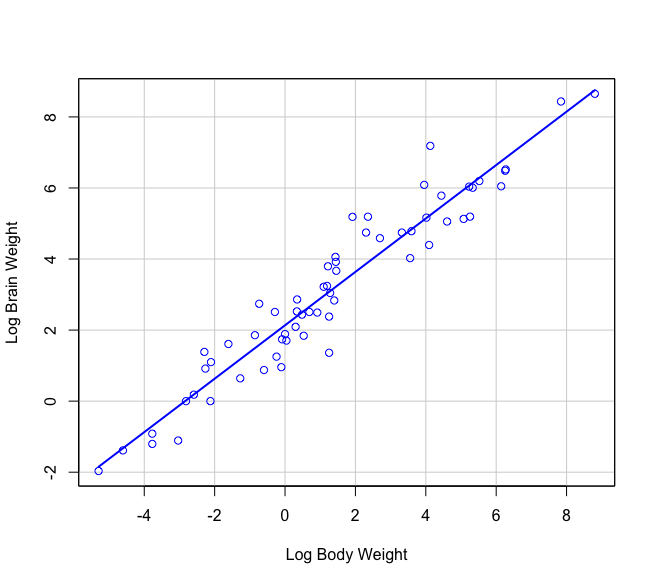
\includegraphics[width=.66\textwidth]{Rplot3.png}
    \end{center}
  \end{figure}

  \textbf{Code:}
  \begin{center}
  \lstinputlisting{r3.txt}
  \end{center} 

  \vspace{.15in}

  \item What do you know about the point defined by the mean of $log(BodyWT)$ and
  the mean of $log(BrainWT)$ related to the fitted model. \\
  \solution We know, by how $\hat{\beta_0}$ is defined that the mean pair $(\bar{x}, \bar{y})$
  lies on the fitted line. 
  \vspace{.15in}

  \item If the errors are normally distributed in the population, what are the distributions of 
  the slope estimator and the error variance estimator. \\
  \solution As discussed in the lecture, if $e_i ~ N(0,\sigma^2)$ for all $i$ we know that the 
  \begin{equation*}
    Y_i ~ N(\hat{\beta_0}+\hat{\beta_1}x_i, \sigma^2)
  \end{equation*}
  Since slope estimator and the error variance estimator are a linear combination with respect to $y_i$
  then they must also be normally distributed. 
  \vspace{.15in}

  \item What is the fitted value for Raccoons? What is the residual?\\
  \solution Computed the fitted sample, using the linear model estimators from r. 
  \begin{equation*}
    \hat{y}_{raccoon} = 2.1347883 + 0.7516861*(log(4.288)) = 3.229108
  \end{equation*}
  Computing the residual, with the given data.
  \begin{equation*}
    e_{raccoon} = |3.229108 - log(39.201)| = 0.439594
  \end{equation*}
  \vspace{.15in}

  \item If a new animal species was sampled, which had a $log(BodyWT)$ of 1.46, would the variance 
  of its prediction error match the variance of the fitted value for the racoons? Why or why not?\\
  \solution  We know that the variance for the fitted value is going to be smaller that the variance of the prediction error.
  This is true by definition and is shown below, where the variance of the fitted value is given by, 
  \begin{equation*}
    V(E(Y)) = V(\hat{y}) = \sigma^2 \left(\frac{1}{n} + \frac{(x - \bar{x})^2}{SXX}\right)
  \end{equation*}
  and the variance of the prediction error is given by, 
  \begin{equation*}
    V(\hat{y} - y^*) =  \sigma^2 \left(1 + \frac{1}{n} + \frac{(x - \bar{x})^2}{SXX}\right)
  \end{equation*}
  This makes sense, as its harder to predict a parameter then it is to estimate one. 


    

    
    
  \end{enumerate}
  
\end{exercise}





\end{document}





















